
\section{Projet OptiHR}
\subsection{Introduction}
L'objectif du projet OptiHR est de développer un logiciel de gestion des \ac{RH} pour l'ARCOP. Cette solution permettra de centraliser et d'automatiser la gestion des congés, des absences, des dossiers personnels et des communications internes.

\subsection{Spécifications fonctionnelles}
\subsubsection{Gestion des Congés et Absences}
\begin{itemize}
    \item \textbf{Mise à jour du planning et du solde des congés} : Demandes de congés en ligne avec circuit de validation (supérieur → GRH → DG)
    \item \textbf{Rapports personnalisables} : Génération de rapports sur la durée, fréquence et motifs des congés
\end{itemize}

\subsubsection{Gestion des dossiers}
\begin{itemize}
    \item \textbf{Dossier personnalisé en ligne} : Accès aux informations personnelles (congés, absences, etc.)
    \item \textbf{Téléchargement des bulletins de paie} : Extraction depuis Sage Paie et mise à disposition
    \item \textbf{Demande de documents administratifs} : Attestations et certificats de travail en ligne
\end{itemize}

\subsubsection{Publication des notes et informations}
\begin{itemize}
    \item \textbf{Diffusion des informations RH} : Publication de notes et documents
    \item \textbf{Alertes et notifications} : Rappels d'échéances et suivi des demandes
\end{itemize}

\subsection{Définition des acteurs systèmes}
Les utilisateurs principaux du système OptiHR sont :
\begin{itemize}
    \item \textbf{Employé} : Personnel de l'ARCOP accédant à ses informations personnelles et effectuant des demandes
    \item \textbf{GRH} : Chef division des ressources humaines et services généraux gérant les demandes et les processus RH
    \item \textbf{DSAF} : Directeur des services administratif et financier, principalement en consultation
    \item \textbf{DG} : Directeur Général validant les demandes et consultant les données stratégiques
\end{itemize}

\subsection{Cas d'utilisation principaux}
\subsubsection{Gestion des Congés et Absences}
\paragraph{Description des cas d'utilisation}
\begin{itemize}
    \item \textbf{Demande de congé} : Soumission avec date, durée et motif
    \item \textbf{Annulation de demande} : Possible avant validation du supérieur
    \item \textbf{Circuit de validation} : Approbation hiérarchique (supérieur → GRH → DG)
    \item \textbf{Consultation et suivi} : Visualisation du solde et historique des congés
    \item \textbf{Génération de documents} : Téléchargement des confirmations et rapports
\end{itemize}

\paragraph{Diagramme de cas d'utilisation}
\begin{figure}[H]
    \centering
    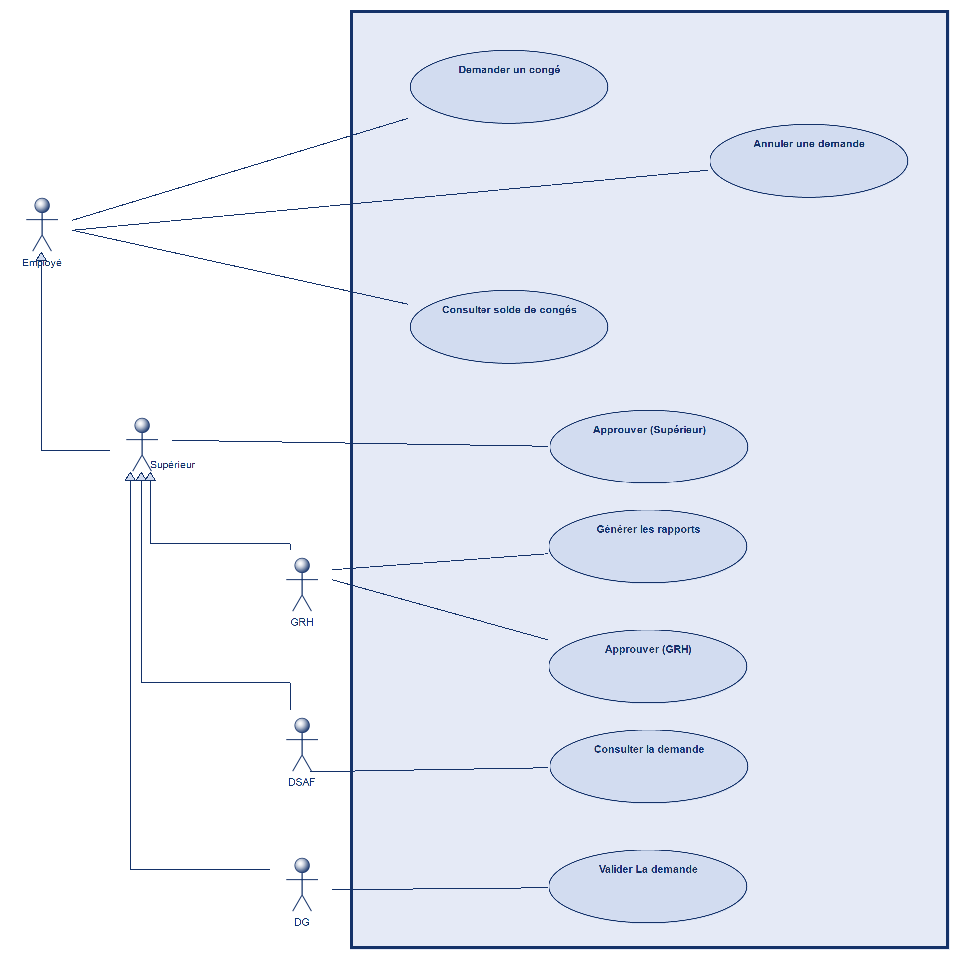
\includegraphics[width=0.8\textwidth]{images/diagrammes/use-cases/conges.png}
    \caption{Diagramme de cas d'utilisation Gestion des Congés et Absences}
    \label{fig:use_case_gestion_conges}
\end{figure}

\paragraph{Diagramme de processus}
\begin{figure}[H]
    \centering
    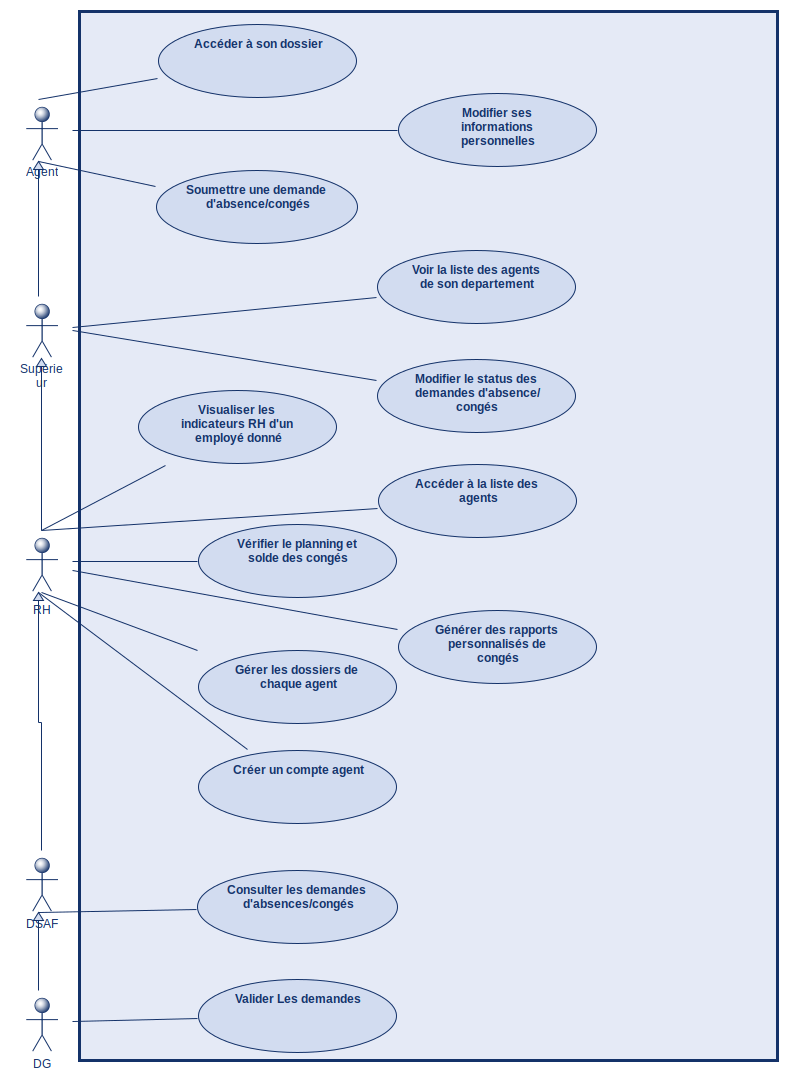
\includegraphics[width=0.8\textwidth]{images/diagrammes/flowcharts/conges.png}
    \caption{Diagramme de processus Gestion des Congés et Absences}
    \label{fig:flow_gestion_conges}
\end{figure}

\subsubsection{Gestion des dossiers}
\paragraph{Description des cas d'utilisation}
\begin{itemize}
    \item \textbf{Consultation du dossier personnel} : Accès aux informations personnelles
    \item \textbf{Téléchargement des bulletins de paie} : Récupération des documents de paie
    \item \textbf{Demande de documents administratifs} : Sollicitation de certificats et attestations
\end{itemize}

\paragraph{Diagramme de cas d'utilisation}
\begin{figure}[H]
    \centering
    \includegraphics[width=0.8\textwidth]{images/diagrammes/use-cases/dossiers.png}
    \caption{Diagramme de cas d'utilisation Gestion des dossiers}
    \label{fig:use_case_gestion_dossiers}
\end{figure}

\paragraph{Diagramme de processus}
\begin{figure}[H]
    \centering
    \includegraphics[width=0.8\textwidth]{images/diagrammes/flowcharts/dossiers.png}
    \caption{Diagramme de processus Gestion des dossiers}
    \label{fig:flow_gestion_dossiers}
\end{figure}

\subsubsection{Publication des notes et informations}
\paragraph{Description des cas d'utilisation}
\begin{itemize}
    \item \textbf{Publication des notes et informations} : Diffusion par le GRH
    \item \textbf{Alertes et notifications} : Système d'information proactif
\end{itemize}

\paragraph{Diagramme de cas d'utilisation}
\begin{figure}[H]
    \centering
    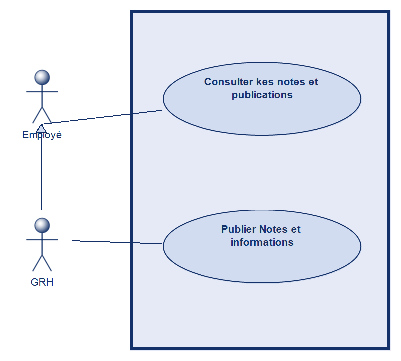
\includegraphics[width=0.8\textwidth]{images/diagrammes/use-cases/note.png}
    \caption{Diagramme de cas d'utilisation Publication des notes et informations}
    \label{fig:use_case_publication}
\end{figure}

\paragraph{Diagramme de processus}
\begin{figure}[H]
    \centering
    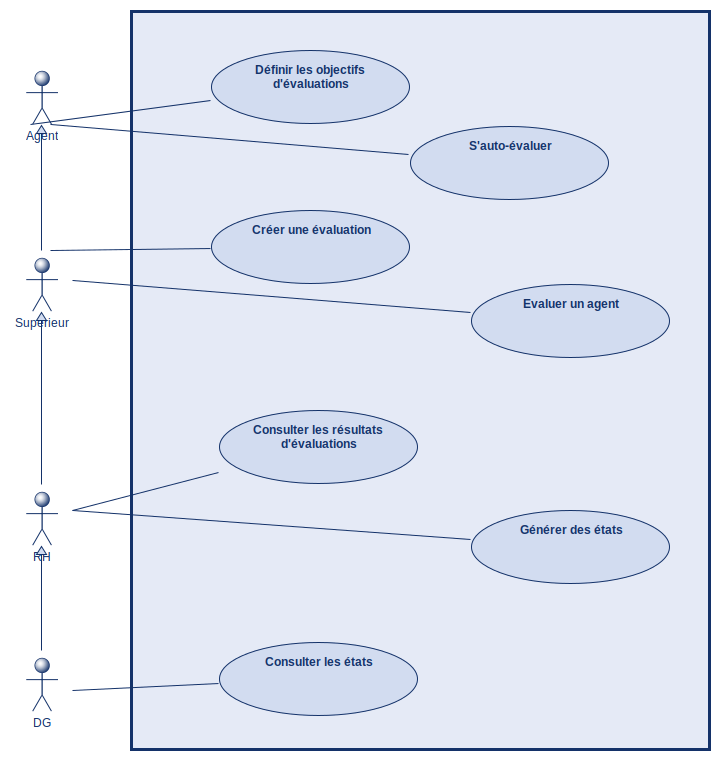
\includegraphics[width=0.8\textwidth]{images/diagrammes/flowcharts/note.png}
    \caption{Diagramme de processus Publication des notes et informations}
    \label{fig:flow_publication}
\end{figure}

